\documentclass[]{beamer}
\usepackage{amssymb,amsmath}
\usepackage{fixltx2e}
\usepackage{lmodern}
\usepackage{tikz}
\IfFileExists{upquote.sty}{\usepackage{upquote}}{}
\IfFileExists{microtype.sty}{\usepackage{microtype}}{}

\usetheme{Warsaw}
\usecolortheme{crane}
\usebackgroundtemplate{%
\tikz\node[opacity=0.2] {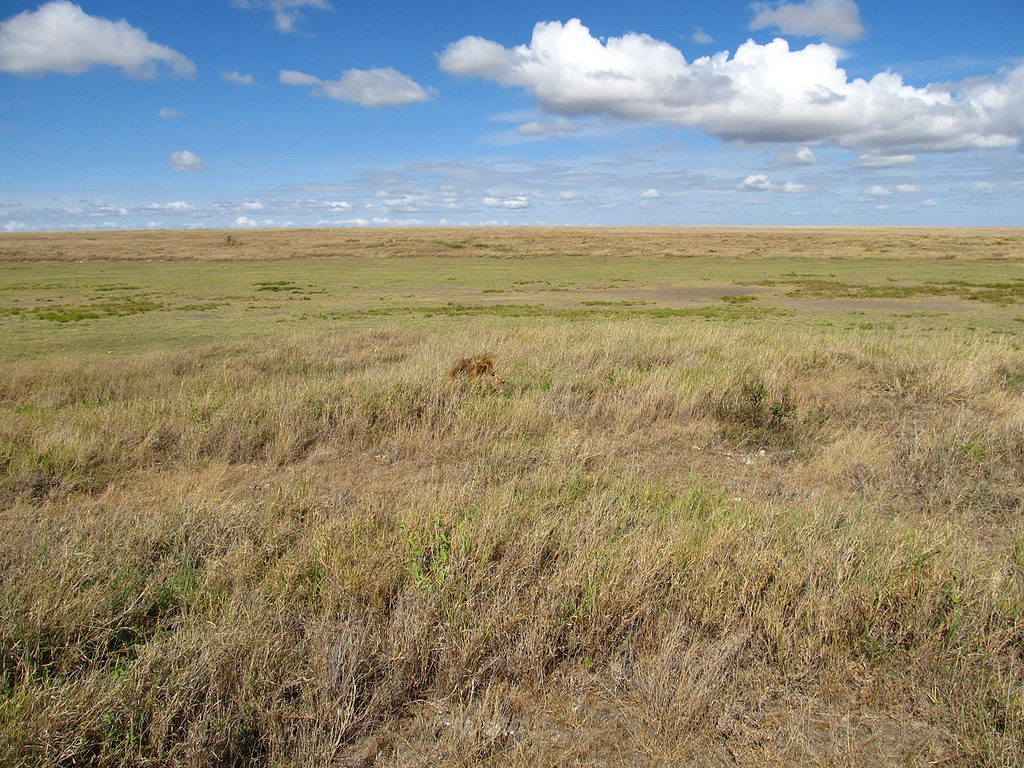
\includegraphics[height=\paperheight,width=\paperwidth]{images/Serengeti_background.jpg}};}

\setbeamercolor{mycolor}{fg=red,bg=olive}

\defbeamertemplate*{footline}{shadow theme}{%
\leavevmode%
\hbox{\begin{beamercolorbox}[wd=.5\paperwidth,ht=2.5ex,dp=1.125ex,leftskip=.3cm plus1fil,rightskip=.3cm]{author in head/foot}%
    \usebeamerfont{author in head/foot}\hfill\insertshortauthor
\end{beamercolorbox}%

\begin{beamercolorbox}[wd=.5\paperwidth,ht=2.5ex,dp=1.125ex,leftskip=.3cm,rightskip=.3cm plus1fil]{title in head/foot}%
    \usebeamerfont{title in head/foot}\insertshorttitle\hfill%
\insertframenumber\,/\,\inserttotalframenumber
\end{beamercolorbox}}%
\vskip0pt%
}

\setlength{\parindent}{0pt}
\setlength{\parskip}{6pt plus 2pt minus 1pt}
\setlength{\emergencystretch}{3em}  % prevent overfull lines
\setcounter{secnumdepth}{0}

\title{Evolving in a tangled world}
\author{Giulio Dalla Riva\\
\tiny{gvd16@uclive.ac.nz}\\
}
\date{  {\tiny Biomathematical Research Centre\\
  University of Canterbury\\
     gvdr.github.io\\
     \vskip 0.5cm
  }
MCEB - June 22, 2015}


\begin{document}
\frame{\titlepage
\addtocounter{framenumber}{-1}}

\begin{frame}{Species are entangled}

\centering
\begin{tabular}{|c|c|}\hline
Evolution & Ecology \\\hline\hline
Phylogeny & Food Web \\
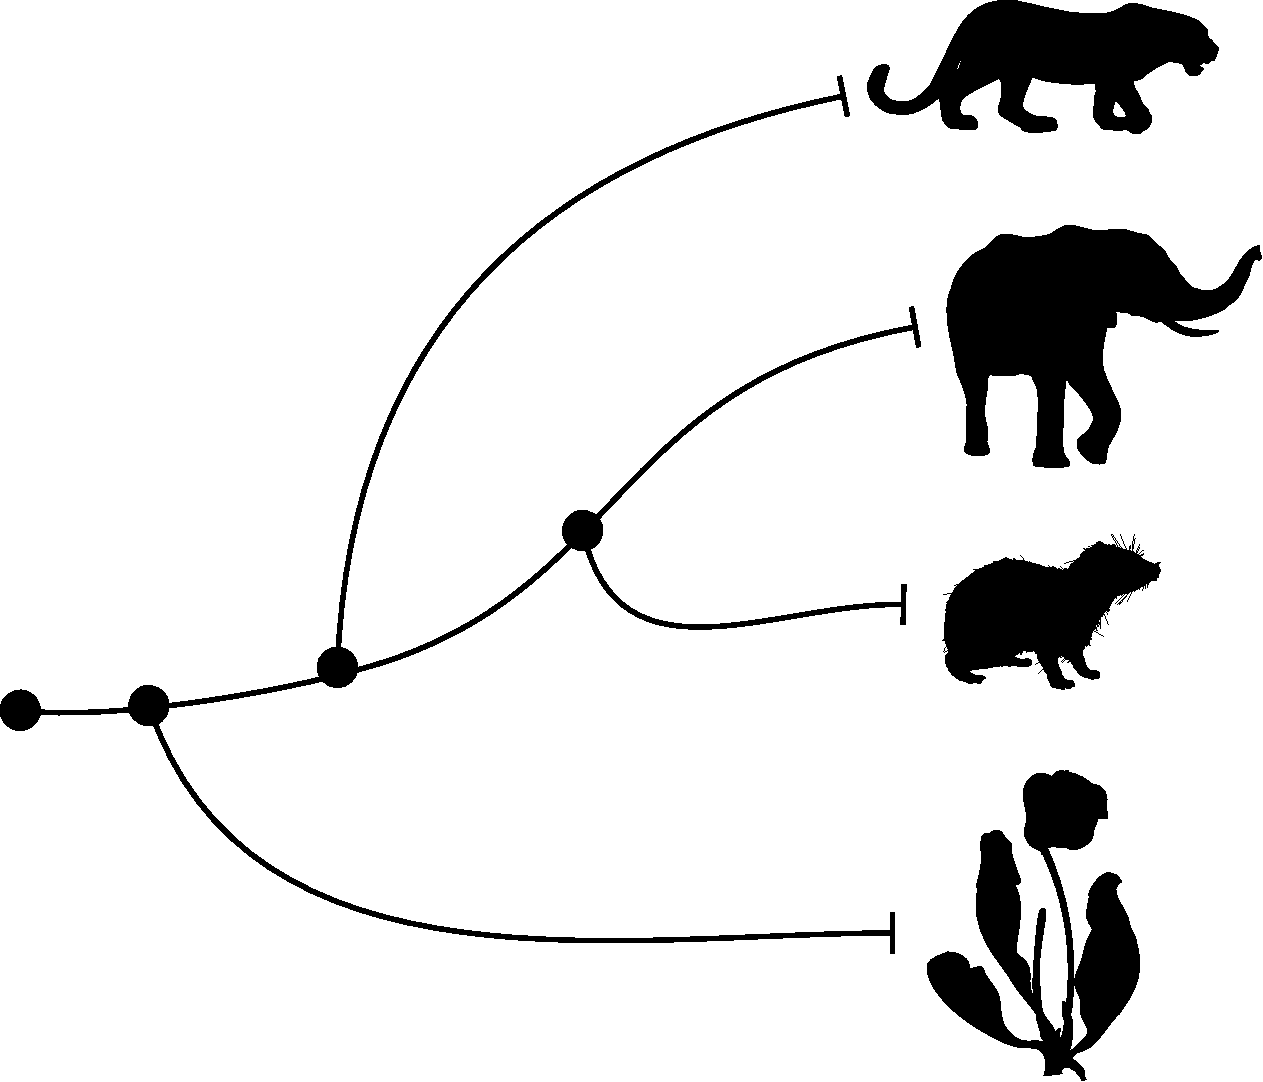
\includegraphics[width=0.4 \textwidth]{images/small_phylo.pdf} & 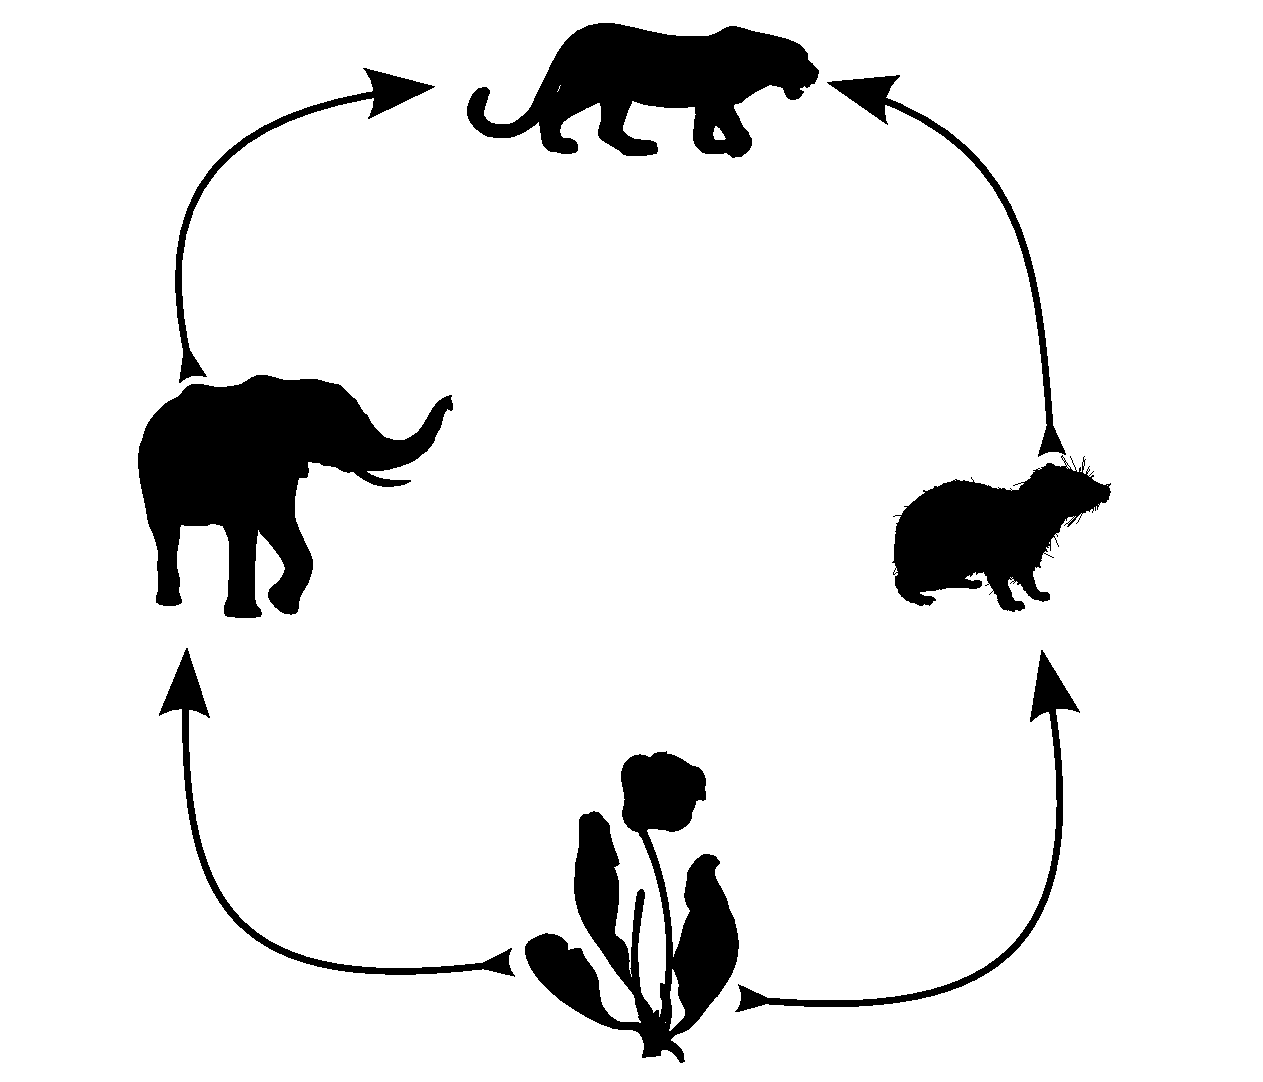
\includegraphics[width=0.4 \textwidth]{images/small_fw.pdf} \\ \hline
\end{tabular}

\end{frame}

\begin{frame}{the Theater and the Play}

\begin{figure}
\centering
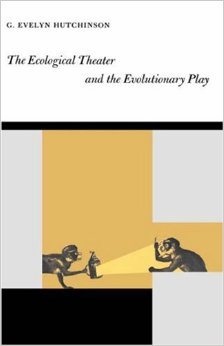
\includegraphics[height=0.5 \textheight]{images/hutchinson_ecotheatreevoplay.jpg}
\end{figure}
\centering
{\tiny Ecology and Evolution occur on different time scales?}

\end{frame}

\begin{frame}{the Theater and the Play}

\begin{figure}
\centering
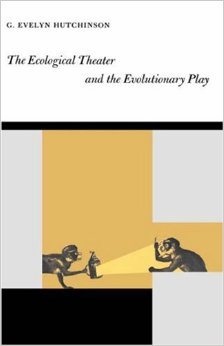
\includegraphics[height=0.5 \textheight]{images/hutchinson_ecotheatreevoplay.jpg}
\end{figure}
\centering
{\tiny Well, maybe, when evolution is really fast...}

\end{frame}

\begin{frame}{A Web on a Tree}

\centering
It's hard to fit a Web on a Tree because of all the fine wirings.

\centering
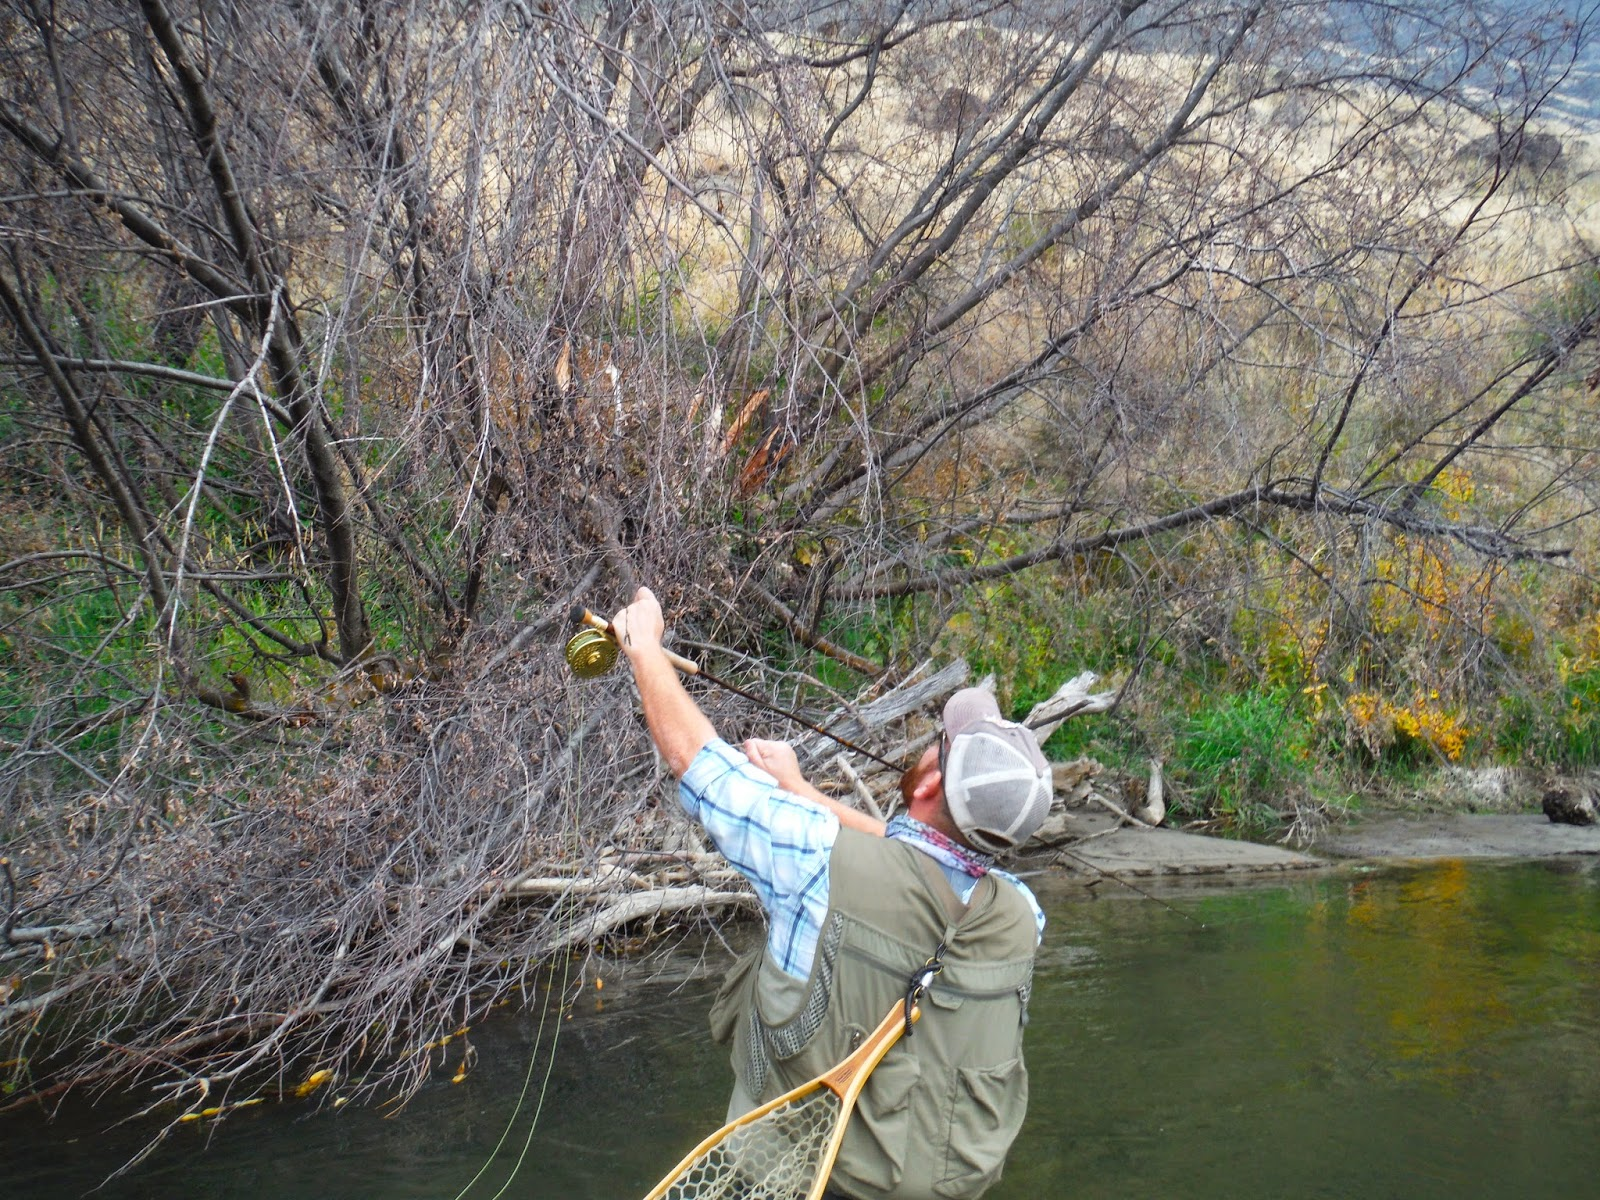
\includegraphics[height=0.5 \textheight]{images/finewirings.jpg}

\centering
{\tiny Courtesy of Erik Moncada}

\end{frame}

\begin{frame}{A Web on a Tree}

\centering
And you don't always get something out of it.

\centering
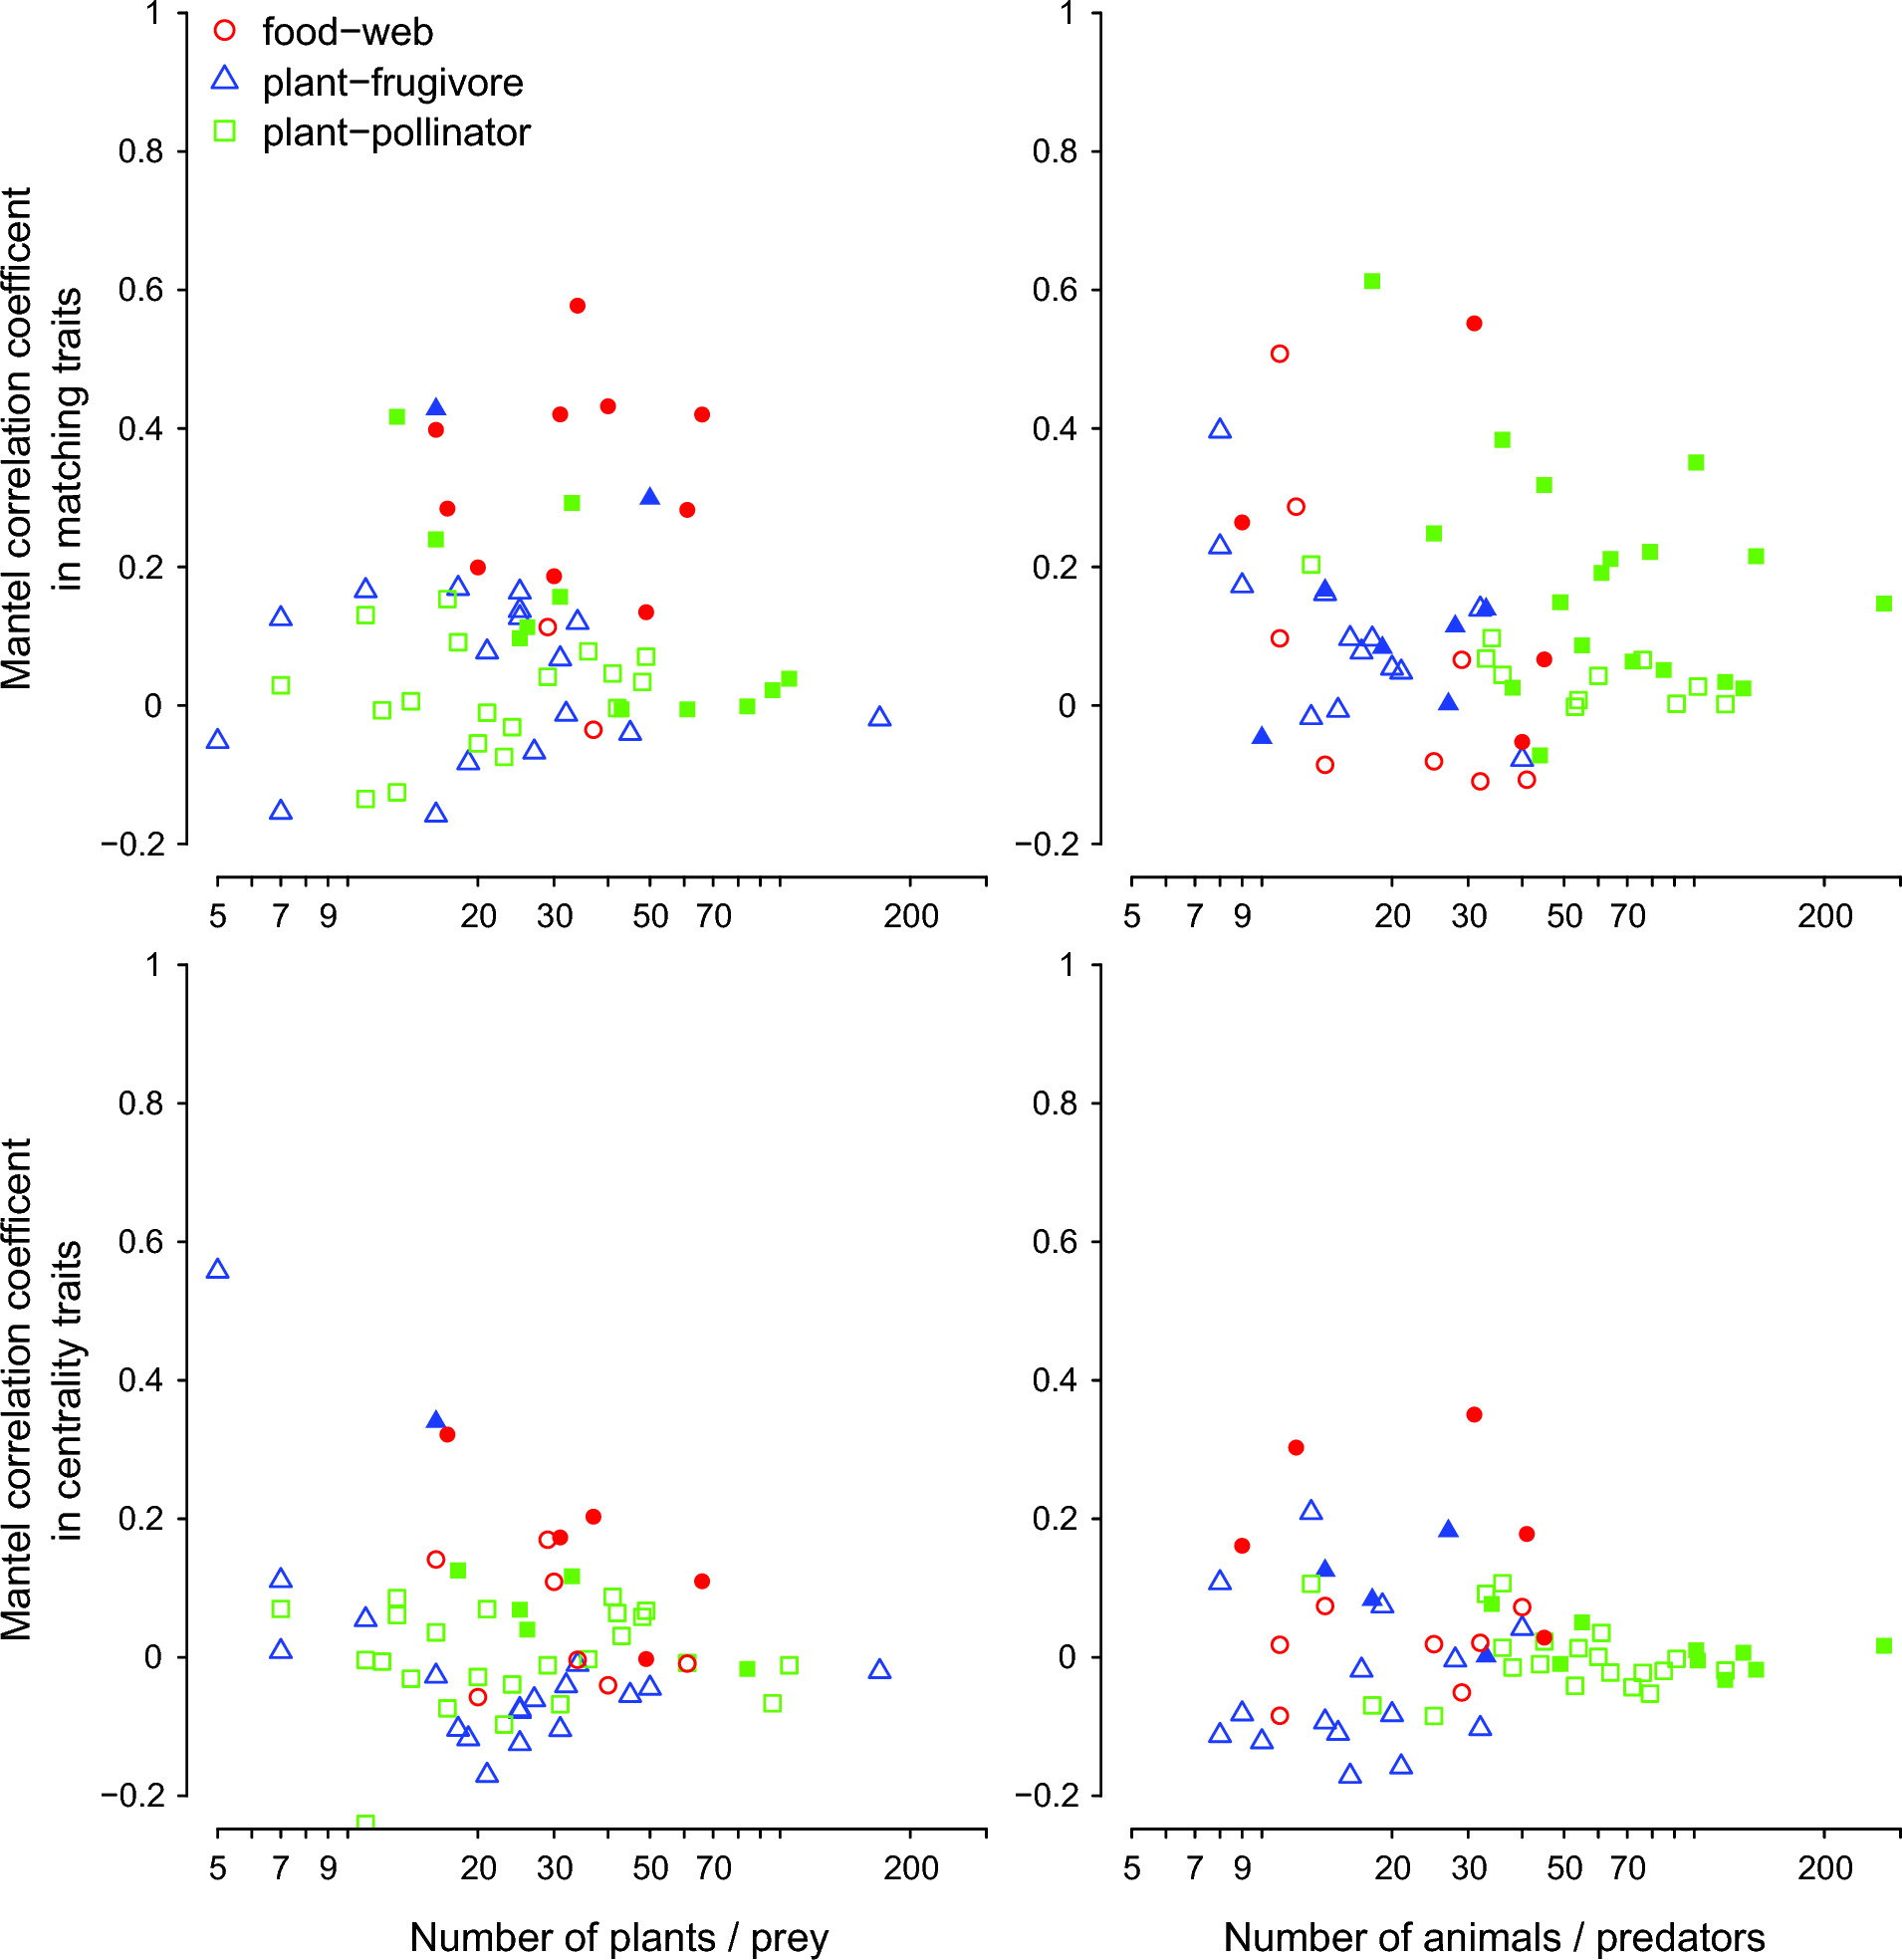
\includegraphics[height=0.7 \textheight]{images/rohr.jpg}

\centering
{\tiny Rohr \& Bascompte, Am Nat 184, 5 (2014)}


\end{frame}


\begin{frame}{A Metric Space on a Tree}

What if we could do without the wiring?

{[}Two images: Serengeti and Weddell{]}

\end{frame}


\begin{frame}{Food Webs embedded}

\centering
\begin{itemize}[<+->]
\itemsep1pt\parskip0pt\parsep0pt
\item
From $G=(V,E)$ to a metric space and back via\\
Random Dot Product Graph
\item
$\mathbb{P}\left( i \to j\right) = \mathbb{T}_{out}\left(i\right) \cdot  \mathbb{T}_{in}\left(j\right)$
\item
SVD(Adjacency) gives $\mathbb{T}_{out}$ and $ \mathbb{T}_{in}$
\end{itemize}

\end{frame}

\begin{frame}{Food Webs embedded}


\centering
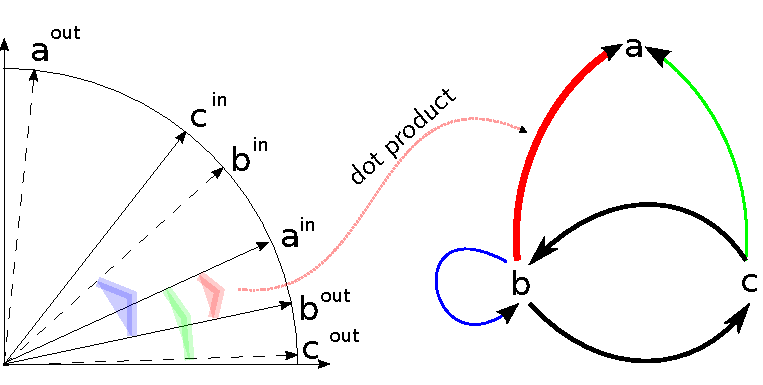
\includegraphics[width=0.6\linewidth]{images/RDPGmodel.pdf}

\centering
{\tiny Three species toy model. gvdr \& Daniel B. Stouffer, appearing}

\end{frame}

\begin{frame}{Food Webs embedded}

\centering
  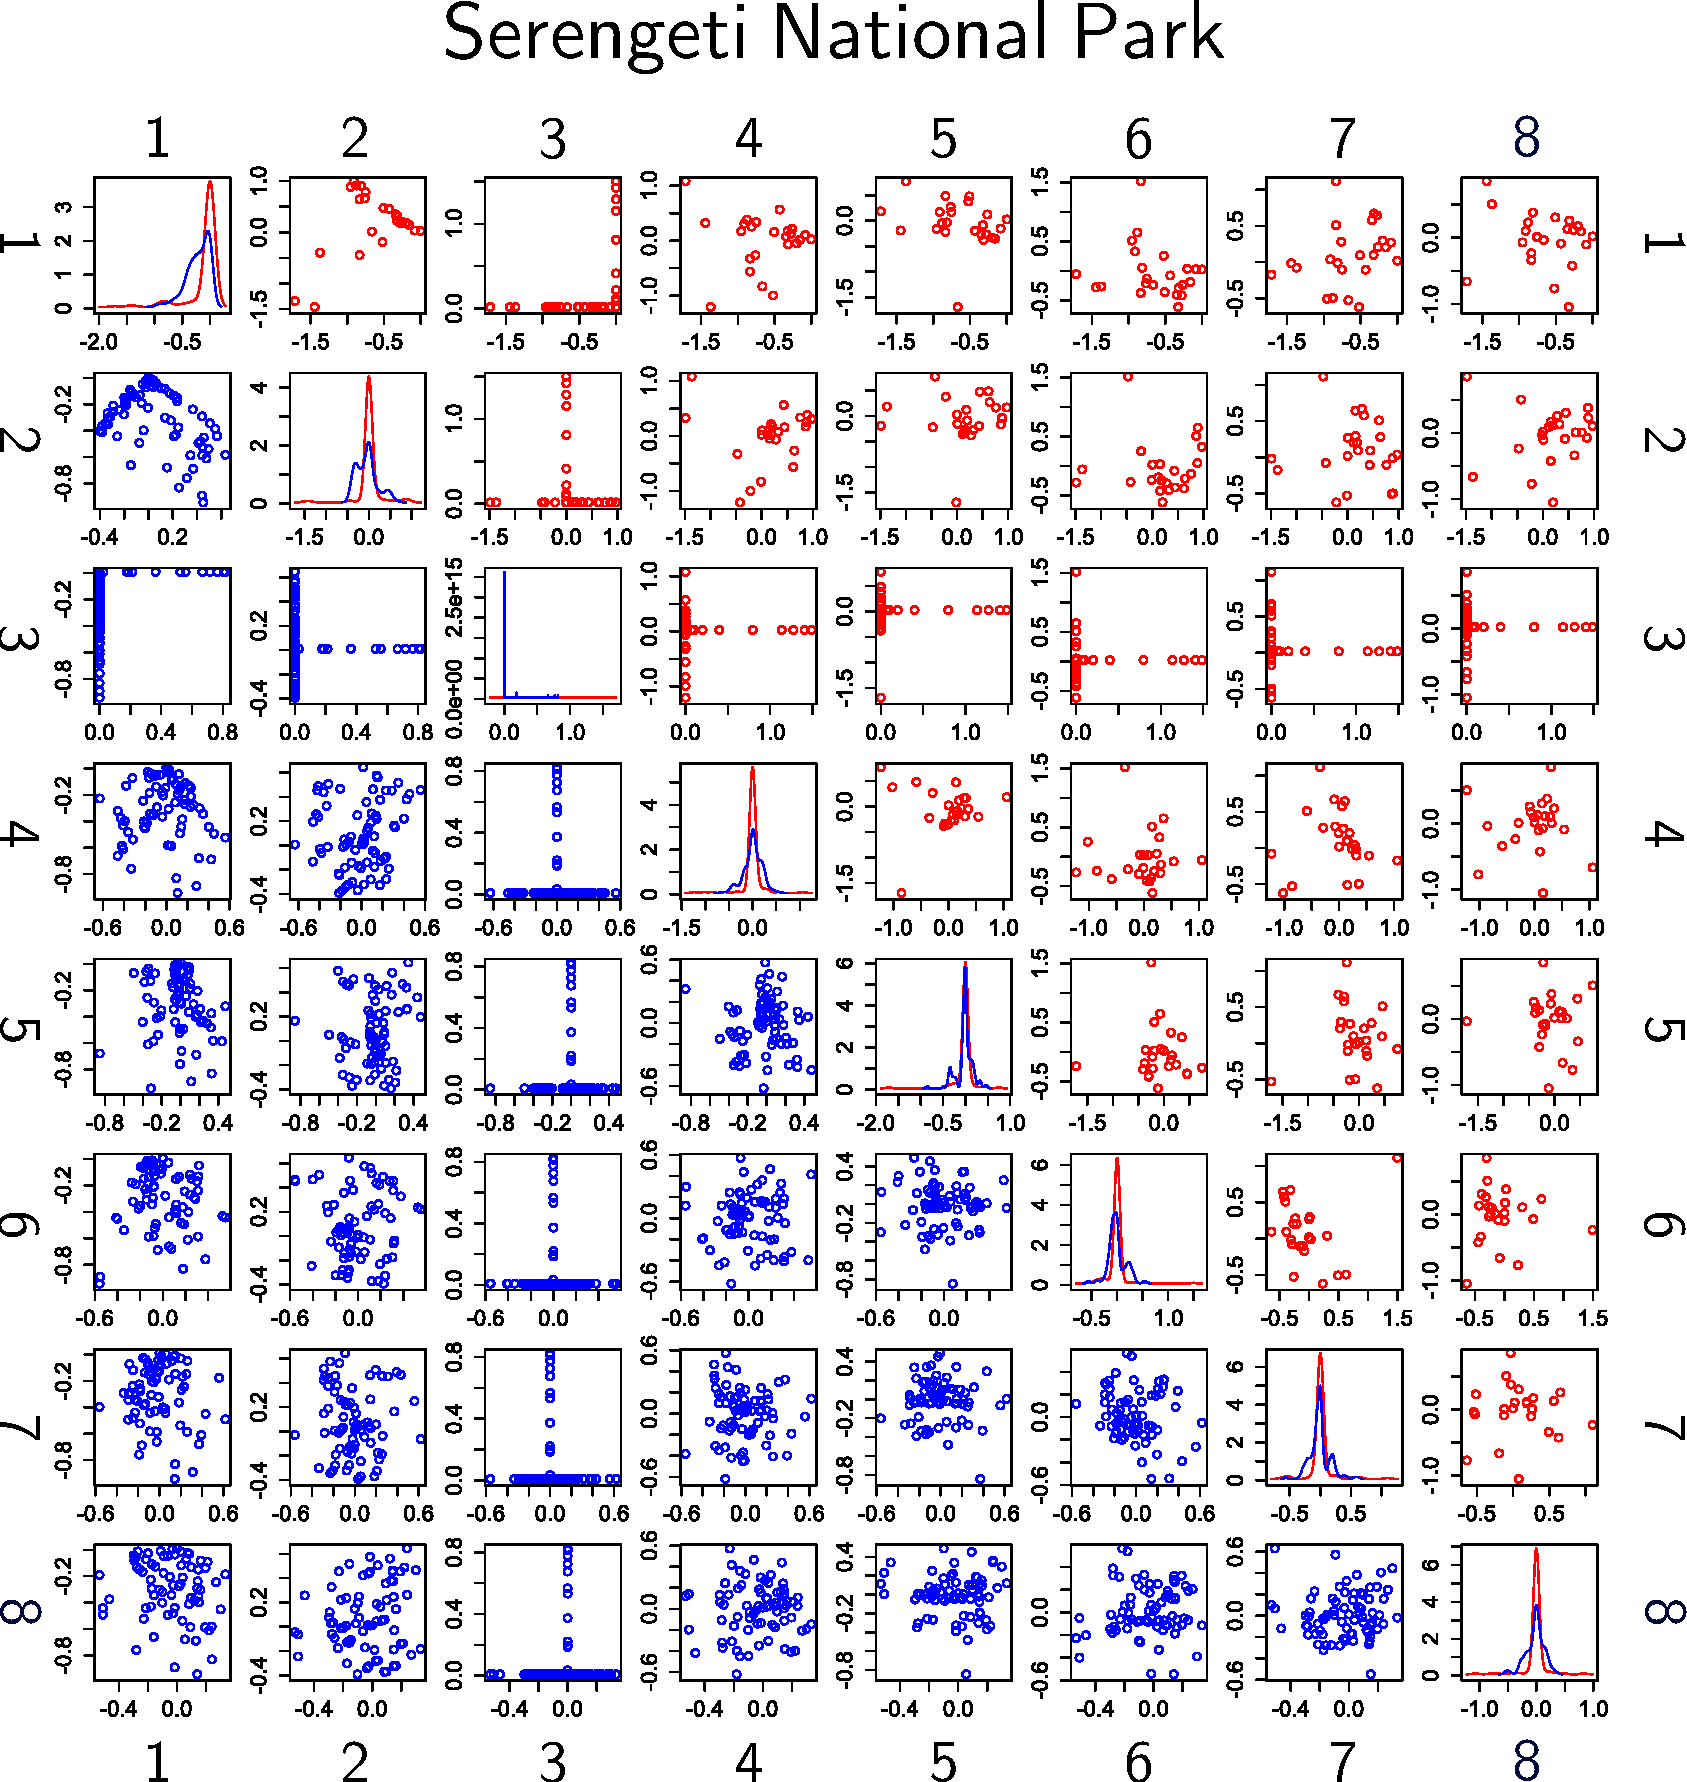
\includegraphics[width=0.6\linewidth]{images/Serengeti_scatter_8.pdf}

\centering
{\tiny A Food Web as you've never seen it}
 
\end{frame}

\begin{frame}{Food Webs embedded}

\centering
  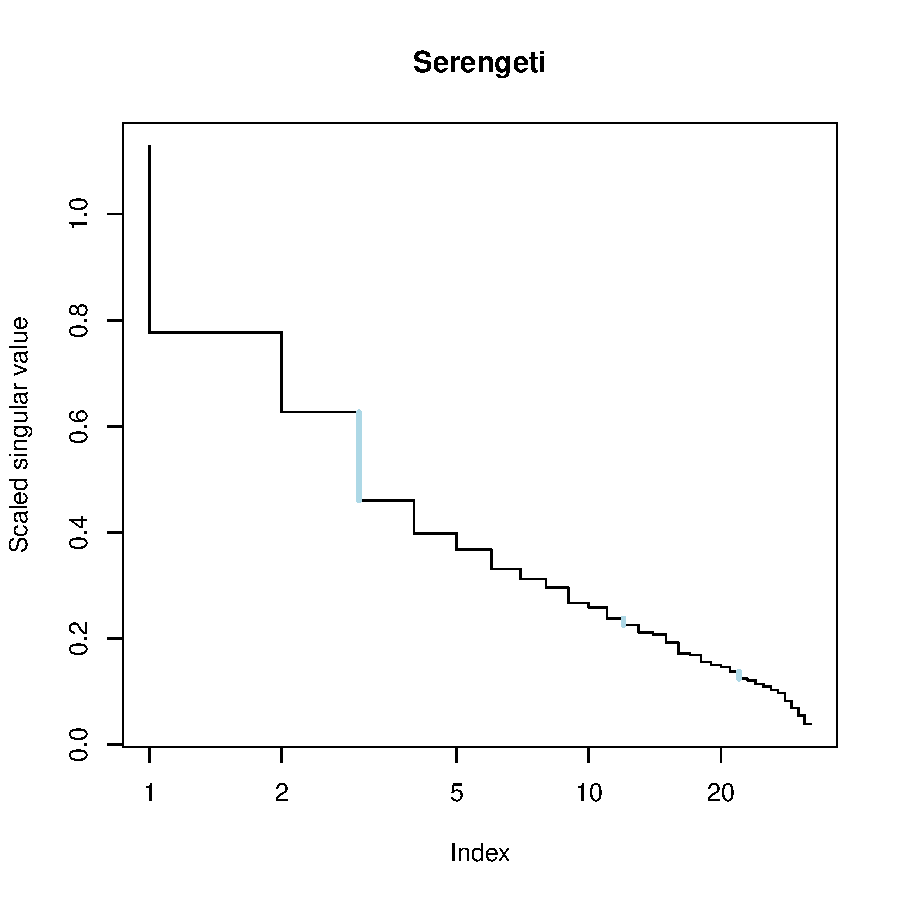
\includegraphics[width=0.4\linewidth]{images/Serengeti_svds.pdf}
  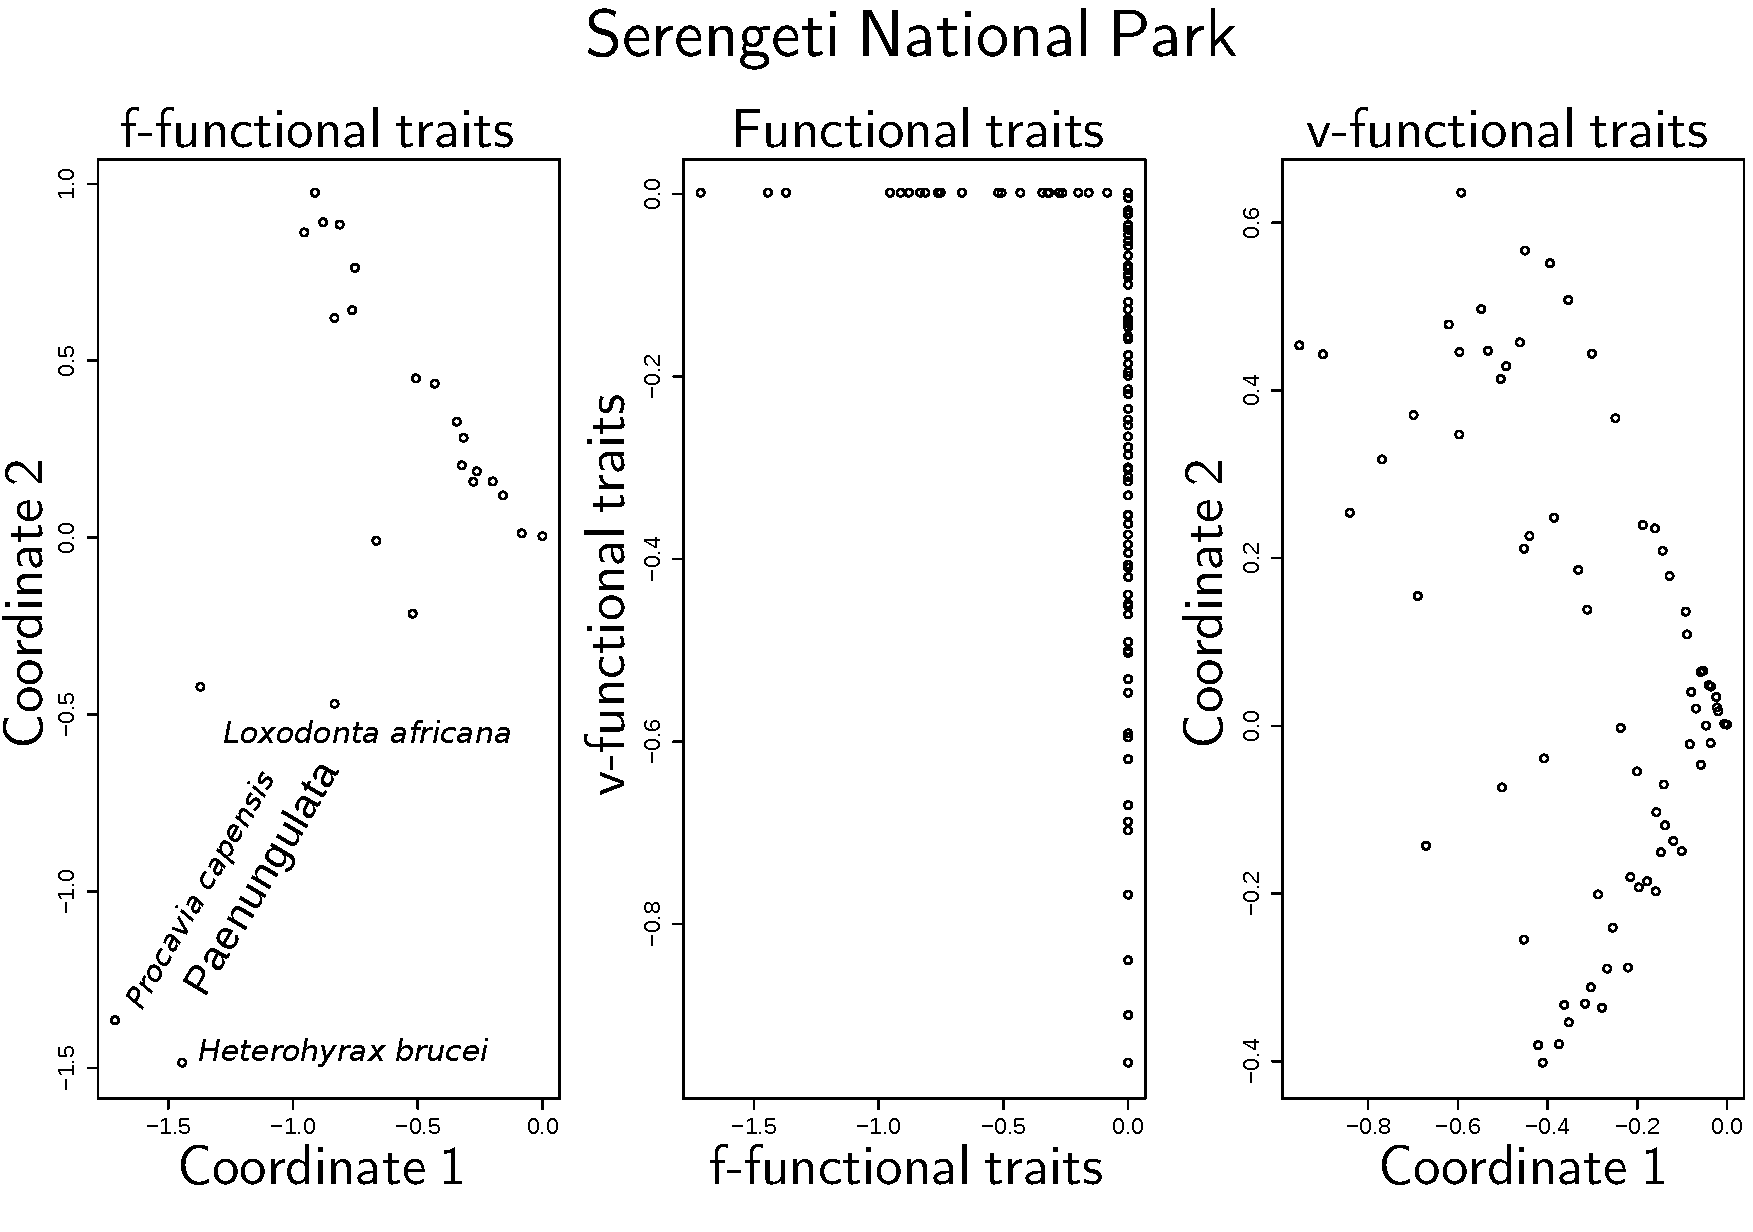
\includegraphics[width=0.6\linewidth]{images/Serengeti_Traits.pdf}

\centering
{\tiny SVDS allows helps in choosing a suitable model dimension.}
 
\end{frame}

\begin{frame}{PCM crash course}

\centering
Observed traits vs. Expectation

  \begin{equation*}
    \textrm{vcv}\left( \hat{x} | \tau, \mbox{null model} \right) \mbox{ vs. } \textrm{vcv}\left(x\right)
  \end{equation*}

\end{frame}

\begin{frame}{PCM crash course}

\centering

\begin{itemize}[<+->]
\itemsep1pt\parskip0pt\parsep0pt
\item
But what null model?
\item
Brownian Motion
\item
Ornstein-Uhlenbeck (BM + rubber band)
\end{itemize}

\end{frame}

\begin{frame}{More questions (than answers)}

\begin{itemize}[<+->]
\itemsep1pt\parskip0pt\parsep0pt
\item
  There is phylogenetic signal\\
  {\tiny p-values anybody?}
\item
  It is quite weak\\
  {\tiny $20\% ~ 30\%$ of variation explained}
\item
  It saturates with dimensionality\\
  {\tiny $d \in \left\{2, \dots , 8 \right\}$}
\item
  $\therefore$ ``fine wirings'' may be deceiving
\item
  Evolutionary model is inadequate\\
  {\tiny no interaction effects}
\end{itemize}

\end{frame}

\begin{frame}{(Not a) Conclusion}

\begin{itemize}[<+->]
\item
  Spoiler 1: Evolutionary distinctiveness vs. Web Centrality\\
  {\small Do evolutionary unique species play a keystone role in Food Webs?}
\item
  Spoiler 2: An ecological informed model of species evolution maybe
  it's (almost) there.\\
  {\small I am looking at you, Ornstein and Uhlenbecki $\dots$}
\end{itemize}

\end{frame}

\begin{frame}{Thanks!}

\begin{centering}

Joint work with  
Daniel B. Stouffer (University of Canterbury)

Many thanks to  
Mike Steel; Carey Priebe; A. Mooers', D.B. Stouffer's \& J. Tylianakis's labs; ...

Funds by the Allan Wilson Centre for Molecular Ecology and Evolution.

\vspace{2cm}

\small{By the way, I'm looking for a postdoc.\\ gvd16@uclive.ac.nz - gvdr.github.io}

\end{centering}

\end{frame}

\end{document}
